\chapter{Het hart en de bloedsomloop}\label{ch:g7:heart-and-circulation}

\Cref{ch:g4:heart-and-blood} stelde de pomp en haar bezorgrondes voor;
sindsdien heeft het \omterm{prop:g4:journey-of-food:absorb}{bloed} er verantwoordelijkheden bij gekregen ---
\omterm{def:g7:digestion-and-nutrients:families}{voedingsstoffen} bij de \omterm{prop:g7:digestion-and-nutrients:absorption}{darmvlokken}
(\cref{prop:g7:digestion-and-nutrients:absorption}), \omterm{def:g7:what-is-respiration:respiration}{zuurstof} bij de
\omterm{def:g7:lungs-and-gas-exchange:alveoli}{longblaasjes} (\cref{prop:g7:lungs-and-gas-exchange:numbers}), rekeningen
bij elke werkende \omterm{def:g3:bones-and-muscles:muscle}{spier} (\cref{prop:g7:organs-at-work:bill}). Tijd om het
wegennet netjes in kaart te brengen: de vier \omterm{def:g7:heart-and-circulation:rooms}{kamers} van het \omterm{def:g4:heart-and-blood:heart}{hart}, de twee
circuits en de drie \omterm{def:g5:biodiversity:species}{soorten} vaten.

\section{De vier kamers van het hart}

\begin{definition}[Boezems en kamers]\label{def:g7:heart-and-circulation:rooms}
De twee helften van het \omterm{def:g4:heart-and-blood:heart}{hart} (\cref{def:g4:heart-and-blood:heart}) hebben
elk twee ruimtes: bovenin een \emph{boezem}\index{boezem} die het
binnenkomende \omterm{prop:g4:journey-of-food:absorb}{bloed} opvangt, en onderin een \emph{kamer}\index{hartkamer}
--- de dikwandige pompruimte --- die het naar buiten drijft. Ertussen en
erachter zitten \emph{kleppen}\index{klep (hart)} --- eenrichtingsdeuren
--- die achter elke stoot dichtklappen; hun paarsgewijze klappen zijn
precies de ``lub-dub'' die een stethoscoop (of een \omterm{def:g1:the-five-senses:sense}{oor} op een borst) hoort.
\end{definition}

\begin{proposition}[Eén slag, op volgorde]\label{prop:g7:heart-and-circulation:beat}
Elke slag doorloopt aan beide kanten tegelijk dezelfde volgorde: de
\omterm{def:g7:heart-and-circulation:rooms}{boezems} trekken samen en vullen de \omterm{def:g7:heart-and-circulation:rooms}{kamers} bij; de \omterm{def:g7:heart-and-circulation:rooms}{kamers} trekken samen en
drijven het \omterm{prop:g4:journey-of-food:absorb}{bloed} naar buiten --- de rechterkant naar de \omterm{def:g7:how-animals-breathe:four}{longen}, de
linkerkant naar het lichaam --- terwijl de instroomkleppen dichtslaan
(lub); de \omterm{def:g7:heart-and-circulation:rooms}{kamers} ontspannen, de uitstroomkleppen slaan dicht (dub), en de
ruimtes vullen zich weer. En dan opnieuw, $100000$ keer per dag
(\cref{rem:g4:heart-and-blood:rest}).
\end{proposition}
\admitted

\section{Twee circuits, drie vaten}

\begin{definition}[De dubbele bloedsomloop]\label{def:g7:heart-and-circulation:double}
Het wegennet van het \omterm{prop:g4:journey-of-food:absorb}{bloed} bestaat uit twee lussen door één pomp (de twee
helften uit \cref{def:g4:heart-and-blood:heart}, nu als circuits):
\begin{itemize}
  \item de \emph{longcirculatie}: rechterkamer $\rightarrow$ \omterm{def:g7:how-animals-breathe:four}{longen}
        (\omterm{def:g7:what-is-respiration:respiration}{zuurstof} laden, \omterm{def:g7:what-is-respiration:respiration}{koolstofdioxide} lossen) $\rightarrow$
        linkerboezem;
  \item de \emph{lichaamscirculatie}: linkerkamer $\rightarrow$ het hele
        lichaam (afleveren, ophalen) $\rightarrow$ rechterboezem.
\end{itemize}
Elke druppel wisselt van circuit: \omterm{def:g7:how-animals-breathe:four}{longen}, lichaam, \omterm{def:g7:how-animals-breathe:four}{longen}, lichaam --- en
daarom is de linkerkamer, die de veel grotere lichaamslus rond moet
duwen, de dikwandigste ruimte van het \omterm{def:g4:heart-and-blood:heart}{hart}.
\end{definition}

\begin{definition}[Slagaders, haarvaten, aders]\label{def:g7:heart-and-circulation:vessels}
Drie \omterm{def:g5:biodiversity:species}{soorten} vaten vormen elke lus
(\cref{def:g4:heart-and-blood:vessels}, nu benoemd):
\begin{itemize}
  \item \emph{slagaders}\index{slagader}: dikwandig, elastisch, en ze
        voeren het \omterm{prop:g4:journey-of-food:absorb}{bloed} onder druk \emph{weg van} het \omterm{def:g4:heart-and-blood:heart}{hart} --- de
        \omterm{prop:g4:heart-and-blood:pulse}{polsslag} (\cref{prop:g4:heart-and-blood:pulse}) is hun oprekken
        bij elke stoot;
  \item \emph{haarvaten}\index{haarvat}: de haarfijne vaatjes die elk
        orgaan doorweven --- met wanden van één \omterm{def:g5:first-look-at-cells:cell}{cel} dik, waar
        \emph{alle} uitwisselingen gebeuren: \omterm{def:g7:lungs-and-gas-exchange:alveoli}{longblaasjes}, \omterm{prop:g7:digestion-and-nutrients:absorption}{darmvlokken},
        \omterm{def:g3:bones-and-muscles:muscle}{spieren}, \omterm{def:g1:the-five-senses:sense}{huid};
  \item \emph{aders}\index{ader}: wijd, dunwandiger, en ze brengen het
        \omterm{prop:g4:journey-of-food:absorb}{bloed} onder lage druk \emph{naar} het \omterm{def:g4:heart-and-blood:heart}{hart} terug, met eigen
        eenrichtingskleppen --- de blauwige lijnen uit
        \cref{rem:g4:heart-and-blood:see}.
\end{itemize}
\end{definition}

\begin{omfigure}
\begin{tikzpicture}[scale=0.9]
  % heart center: four rooms
  \draw[thick] (3.8,2.1) rectangle (7.0,3.9);
  \draw[thick] (5.4,2.1) -- (5.4,3.9);
  \draw[thick] (3.8,3.0) -- (7.0,3.0);
  \node[font=\footnotesize, align=center] at (4.6,3.45)
    {rechter-\\ boezem};
  \node[font=\footnotesize, align=center] at (6.2,3.45)
    {linker-\\ boezem};
  \node[font=\footnotesize, align=center] at (4.6,2.55)
    {rechter-\\ kamer};
  \node[font=\footnotesize, align=center] at (6.2,2.55)
    {linker-\\ kamer};
  % lungs above
  \draw[thick, fill=omDef!8] (4.5,5.2) ellipse (0.75 and 0.6);
  \draw[thick, fill=omDef!8] (6.3,5.2) ellipse (0.75 and 0.6);
  \node[font=\footnotesize] at (5.4,5.95) {de longen};
  % body below
  \draw[thick, fill=omProp!8, rounded corners=6pt]
    (3.9,-0.7) rectangle (6.9,0.5);
  \node[font=\footnotesize] at (5.4,-0.1) {het hele lichaam};
  % lung circuit arrows
  \draw[->, very thick, omDef] (4.9,3.9) .. controls (4.6,4.4)
    .. (4.5,4.6);
  \draw[->, very thick, omThm] (6.3,4.6) .. controls (6.2,4.35)
    .. (5.95,3.92);
  \node[font=\footnotesize, omDef, left] at (4.35,4.45)
    {om zuurstof te laden};
  % body circuit arrows
  \draw[->, very thick, omThm] (5.95,2.1) .. controls (6.3,1.3)
    .. (6.2,0.52);
  \draw[->, very thick, omDef] (4.6,0.52) .. controls (4.5,1.3)
    .. (4.9,2.08);
  \node[font=\footnotesize, omThm, right] at (6.45,1.3)
    {leveringen eruit};
  \node[font=\footnotesize, omDef, left] at (4.3,1.3)
    {retour erin};
\end{tikzpicture}

{\small De dubbele bloedsomloop: de rechterkant naar de \omterm{def:g7:how-animals-breathe:four}{longen} en terug
naar links; de linkerkant het lichaam rond en terug naar rechts. De rode
pijlen dragen de zuurstofrijke stukken, de blauwe de terugkerende.}
\end{omfigure}

\begin{example}[Eén druppel, één volledige rondrit]\label{ex:g7:heart-and-circulation:tour}
De bezorgronde uit \cref{ex:g4:heart-and-blood:round}, met de namen van de
kaart erbij: rechterkamer --- de \omterm{def:g7:heart-and-circulation:vessels}{haarvaten} van de \omterm{def:g7:how-animals-breathe:four}{long} (\omterm{def:g7:what-is-respiration:respiration}{zuurstof} aan
boord bij de \omterm{def:g7:lungs-and-gas-exchange:alveoli}{longblaasjes}, helderrood) --- linkerboezem, linkerkamer ---
\omterm{def:g7:heart-and-circulation:vessels}{slagader} --- de \omterm{def:g7:heart-and-circulation:vessels}{haarvaten} van een dijspier (\omterm{def:g7:what-is-respiration:respiration}{zuurstof} en \omterm{prop:g7:organs-at-work:bill}{glucose} eraf,
\omterm{def:g7:what-is-respiration:respiration}{koolstofdioxide} erop, donkerder) --- \omterm{def:g7:heart-and-circulation:vessels}{ader}, met \omterm{def:g7:heart-and-circulation:rooms}{kleppen} die de klim
verlichten --- rechterboezem. Twee circuits, binnen een minuut, en geen
verkeerde afslagen beschikbaar: daar zorgen de \omterm{def:g7:heart-and-circulation:rooms}{kleppen} voor.
\end{example}

\begin{remark}[Waarom het om de haarvaten draait]\label{rem:g7:heart-and-circulation:capillaries}
\omterm{def:g7:heart-and-circulation:vessels}{Slagaders} en \omterm{def:g7:heart-and-circulation:vessels}{aders} zijn alleen maar snelwegen; elke werkelijke levering
--- elke uitwisseling die dit jaar bestudeerd heeft --- gebeurt door
haarvatwanden heen. Het bestek uit
\cref{prop:g7:how-animals-breathe:spec} woont ook hier: wanden van één \omterm{def:g5:first-look-at-cells:cell}{cel}
(dun), die elk weefsel met tienduizenden kilometers doorweven
(\cref{def:g4:heart-and-blood:vessels} --- groot), badend in het vocht van
het lichaam. Het \omterm{def:g4:heart-and-blood:heart}{hart} bestaat om het \omterm{prop:g4:journey-of-food:absorb}{bloed} \emph{door de \omterm{def:g7:heart-and-circulation:vessels}{haarvaten}} in
beweging te houden; al het andere is leidingwerk ernaartoe en ervandaan.
\end{remark}

\section{Het net lezen en onderhouden}

\begin{example}[Metingen langs de weg]\label{ex:g7:heart-and-circulation:measures}
Drie alledaagse aflezingen van het net: de \emph{\omterm{prop:g4:heart-and-blood:pulse}{polsslag}} --- het
oprekken van een \omterm{def:g7:heart-and-circulation:vessels}{slagader}, waarmee je de stoten telt
(\cref{met:g4:heart-and-blood:pulse}); de \emph{bloeddruk}, de twee
getallen van de manchet --- de slagaderdruk tijdens de stoot en ertussen;
en de \emph{lub-dub} van de stethoscoop --- de deuren van de \omterm{def:g7:heart-and-circulation:rooms}{kleppen} die
je hoort sluiten. Drie vensters, zonder één snee.
\end{example}

\begin{omfigure}
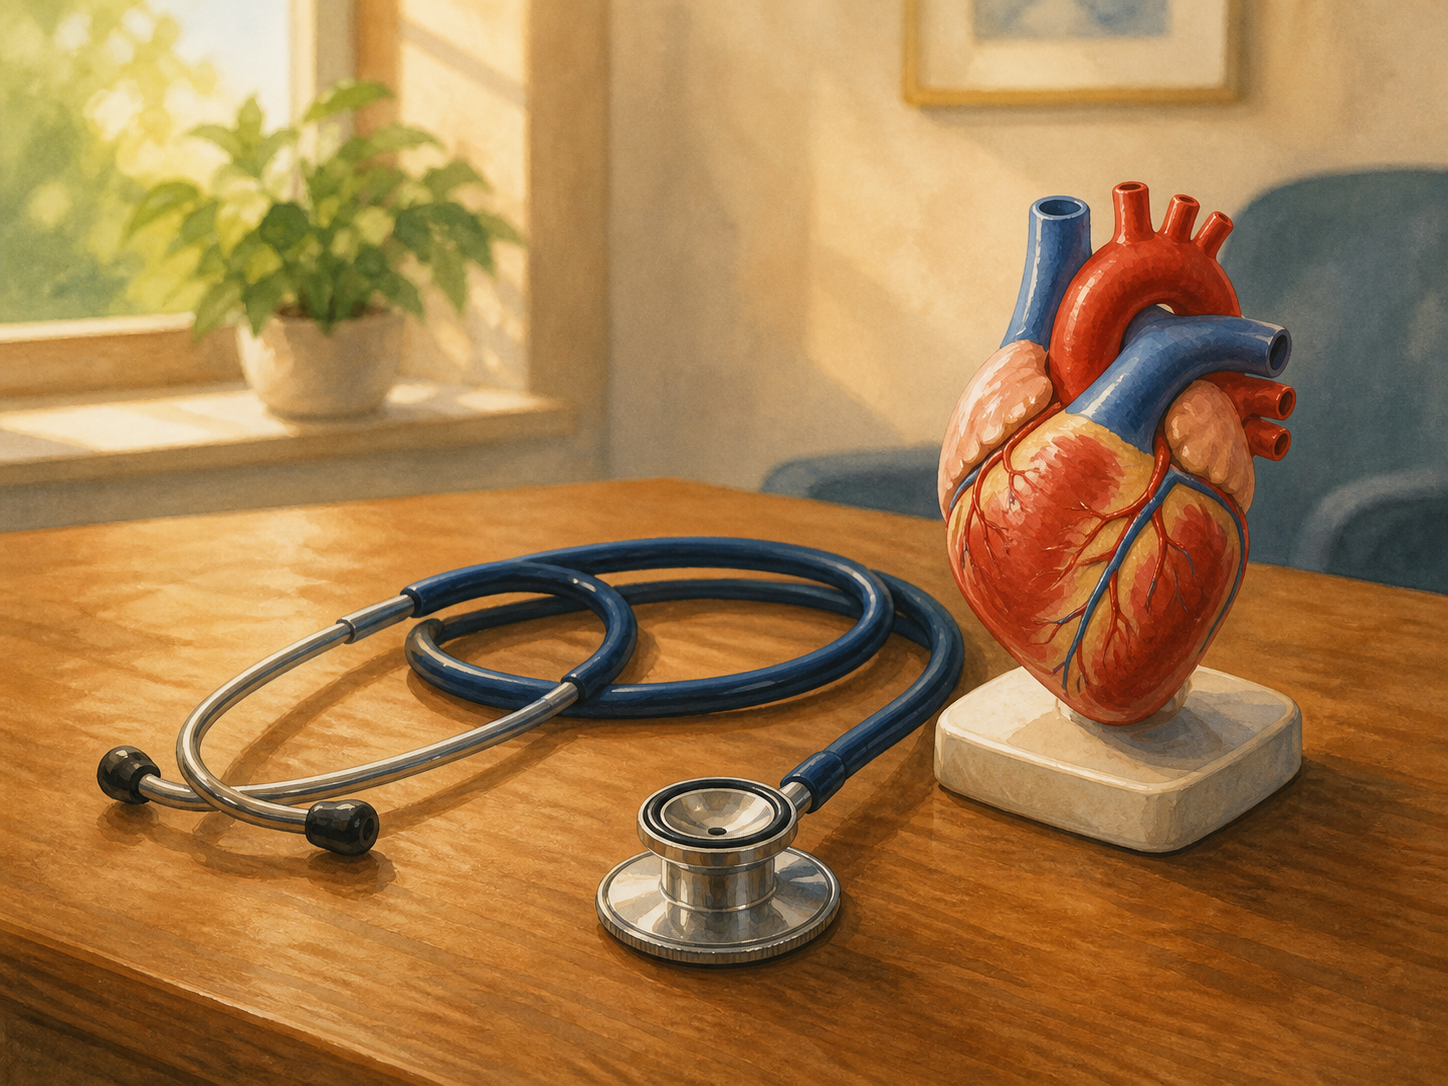
\includegraphics[width=0.56\linewidth]{images/book1/ai/g7-heart-stethoscope.png}

{\small De twee klassiekers van het consult: het model dat de \omterm{def:g7:heart-and-circulation:rooms}{kamers} en de
vaten laat zien, en de stethoscoop die hun deuren hoort dichtvallen.}
\end{omfigure}

\begin{proposition}[Het net onderhouden]\label{prop:g7:heart-and-circulation:keep}
De vijanden en vrienden van het net op lange termijn zijn bekend:
\begin{itemize}
  \item \emph{beweging} versterkt de pomp
        (\cref{prop:g7:organs-at-work:training}) en houdt de snelwegen
        soepel;
  \item \emph{evenwichtig eten}
        (\cref{met:g3:balanced-diet:check}) beschermt de wanden van de
        \omterm{def:g7:heart-and-circulation:vessels}{slagaders}, die door te rijk \omterm{prop:g4:journey-of-food:absorb}{bloed} langzaam dichtslibben en stijf
        worden;
  \item \emph{rook} valt naast de \omterm{def:g7:how-animals-breathe:four}{longen} ook de vaten aan
        (\cref{prop:g7:lungs-and-gas-exchange:smoke}) --- vernauwen,
        verstijven, stoelen stelen;
  \item en de eigen aanvoer van het \omterm{def:g4:heart-and-blood:heart}{hart} --- het voedt zichzelf via eigen
        kleine \omterm{def:g7:heart-and-circulation:vessels}{slagaders}, niet uit het \omterm{prop:g4:journey-of-food:absorb}{bloed} in zijn ruimtes --- hangt van
        alle drie af.
\end{itemize}
De gewoonten uit \cref{prop:g5:healthy-choices:contract} zijn, concreet
gezegd, vaatonderhoud.
\end{proposition}
\admitted

\begin{method}[Elk orgaan in het net inpassen]\label{met:g7:heart-and-circulation:map}
Voor elk orgaan dat dit boek tegenkomt:
\begin{enumerate}
  \item plaats het op de lichaamscirculatie: \omterm{def:g7:heart-and-circulation:vessels}{slagader} erin, \omterm{def:g7:heart-and-circulation:vessels}{ader} eruit,
        \omterm{def:g7:heart-and-circulation:vessels}{haarvaten} erbinnen;
  \item noem wat er door zijn haarvatwanden oversteekt, naar binnen en
        naar buiten (\omterm{prop:g7:digestion-and-nutrients:absorption}{darmvlokken}: \omterm{def:g7:digestion-and-nutrients:families}{voedingsstoffen} naar binnen; \omterm{def:g3:bones-and-muscles:muscle}{spier}:
        brandstof en \omterm{def:g7:what-is-respiration:respiration}{zuurstof} naar binnen, \omterm{def:g7:what-is-respiration:respiration}{koolstofdioxide} naar buiten;
        \omterm{def:g1:the-five-senses:sense}{huid}: warmte naar buiten);
  \item noteer zijn bijzondere aansluiting, als die er is (het \omterm{prop:g4:journey-of-food:absorb}{bloed} van
        de darm gaat eerst bij de \omterm{prop:g7:digestion-and-nutrients:absorption}{lever} langs; de \omterm{def:g7:how-animals-breathe:four}{longen} liggen op hun
        eigen circuit);
  \item toets de stromen aan de taak van het orgaan --- het netwerkschema
        hoort het hoofdstuk over dat orgaan opnieuw te vertellen.
\end{enumerate}
\end{method}

\section{Oefeningen}

\begin{exercise}[$\star$]\label{exo:g7:heart-and-circulation:1}
Noem de vier ruimtes van het \omterm{def:g4:heart-and-blood:heart}{hart} en de rol van elk.
\end{exercise}

\begin{exercise}[$\star$]\label{exo:g7:heart-and-circulation:2}
Waar dienen de \omterm{def:g7:heart-and-circulation:rooms}{kleppen} van het \omterm{def:g4:heart-and-blood:heart}{hart} voor, en wat is de lub-dub?
\end{exercise}

\begin{exercise}[$\star$]\label{exo:g7:heart-and-circulation:3}
Volg de twee circuits, met voor elk het begin, de bestemming en de
terugkeer.
\end{exercise}

\begin{exercise}[$\star$]\label{exo:g7:heart-and-circulation:4}
Geef de drie \omterm{def:g5:biodiversity:species}{soorten} vaten met van elk één bouwkenmerk en één taak.
\end{exercise}

\begin{exercise}[$\star$]\label{exo:g7:heart-and-circulation:5}
Waarom is de linkerkamer de dikwandigste ruimte?
\end{exercise}

\begin{exercise}[$\star$]\label{exo:g7:heart-and-circulation:6}
Waar --- in welke \omterm{def:g5:biodiversity:species}{soort} vaten --- gebeuren alle uitwisselingen van het
lichaam? Noem de haarvatuitwisselingen van drie organen.
\end{exercise}

\begin{exercise}[$\star\star$]\label{exo:g7:heart-and-circulation:7}
Laat \cref{ex:g7:heart-and-circulation:tour} lopen voor een druppel die de
\omterm{def:g5:brain-in-command:system}{hersenen} bedient in plaats van de dij. Wat neemt en wat laat de
haarvatuitwisseling van de \omterm{def:g5:brain-in-command:system}{hersenen} achter?
(\cref{prop:g5:brain-in-command:protect} noemt hun behoeften.)
\end{exercise}

\begin{exercise}[$\star\star$]\label{exo:g7:heart-and-circulation:8}
De \omterm{prop:g4:heart-and-blood:pulse}{polsslag} voel je bij \omterm{def:g7:heart-and-circulation:vessels}{slagaders}, nooit bij \omterm{def:g7:heart-and-circulation:vessels}{aders}. Verklaar dat met de
bouw en de druk van de twee vaten.
\end{exercise}

\begin{exercise}[$\star\star$]\label{exo:g7:heart-and-circulation:9}
\omterm{def:g7:heart-and-circulation:vessels}{Aders} hebben eenrichtingskleppen, \omterm{def:g7:heart-and-circulation:vessels}{slagaders} niet. Welk probleem lossen de
aderkleppen op --- en waarom vallen soldaten die doodstil staan soms flauw?
\end{exercise}

\begin{exercise}[$\star\star$]\label{exo:g7:heart-and-circulation:10}
Pas \cref{met:g7:heart-and-circulation:map} toe op de \omterm{def:g4:journey-of-food:tract}{dunne darm}, met de
bijzondere aansluiting erbij.
\end{exercise}

\begin{exercise}[$\star\star$]\label{exo:g7:heart-and-circulation:11}
Waarom heeft het \omterm{def:g4:heart-and-blood:heart}{hart} eigen kleine voedingsslagaders nodig terwijl zijn
ruimtes vol \omterm{prop:g4:journey-of-food:absorb}{bloed} staan? En waarom doet het dichtslibben ervan er zo veel
toe?
\end{exercise}

\begin{exercise}[$\star\star\star$]\label{exo:g7:heart-and-circulation:12}
``Het \omterm{def:g4:heart-and-blood:heart}{hart} is leidingwerk in dienst van de \omterm{def:g7:heart-and-circulation:vessels}{haarvaten}.'' Verdedig die
bewering met \cref{rem:g7:heart-and-circulation:capillaries} en twee
uitwisselingen uit eerdere hoofdstukken.
\end{exercise}

\section{Probleem: De ochtend van de cardioloog}

\begin{problem}[{Weekendprobleem --- vier consulten, één kaart van het
net}]\label{pb:g7:heart-and-circulation:1}
Loop een ochtend lang mee met een cardioloog voor vier (verzonnen)
consulten, met de kaart in de hand.

\medskip\noindent\textbf{Deel I --- De gezonde
uitgangswaarde.}
\begin{enumerate}
  \item Patiënt 1, een fitte tiener, krijgt de drie aflezingen langs de
        weg uit \cref{ex:g7:heart-and-circulation:measures}. Noem elk, en
        welk deel van de machinerie elk afleest.
  \item Haar \omterm{prop:g4:heart-and-blood:pulse}{polsslag} in rust is $58$. De cardioloog glimlacht. Waarom
        (\cref{exo:g4:heart-and-blood:11})?
  \item Haar lub-dub is helder en dubbel. Wat klapte er precies, twee
        keer, bij elke slag?
  \item Schets de weg van haar \omterm{prop:g4:journey-of-food:absorb}{bloed} vanaf de rechterboezem door allebei
        de circuits en terug, in acht benoemde haltes.
\end{enumerate}

\medskip\noindent\textbf{Deel II --- Drie problemen.}
\begin{enumerate}[resume]
  \item Patiënt 2 heeft een lekkende klep tussen linkerboezem en
        linkerkamer: bij elke slag stroomt er wat \omterm{prop:g4:journey-of-food:absorb}{bloed} terug, met een
        ruisende bijgeruis. Voorspel de gevolgen voor de leveringen van
        de lichaamscirculatie en voor het uithoudingsvermogen van de
        patiënt.
  \item Patiënt 3, een zware roker met een rijk dieet, heeft
        dichtgeslibde, verstijfde \omterm{def:g7:heart-and-circulation:vessels}{slagaders}. Welke aflezingen van consult
        1 zullen verslechterd zijn, en waarom draait de linkerkamer
        overuren?
  \item Het dichtslibben van patiënt 3 betreft ook de eigen
        voedingsslagaders van het \omterm{def:g4:heart-and-blood:heart}{hart}. Leg de bijzondere zorg van de
        cardioloog in één zin uit.
  \item Patiënt 4 heeft dikke enkels na lange dagen staan: de klim
        omhoog van de \omterm{def:g7:heart-and-circulation:vessels}{aders} schiet tekort. Welke onderdelen falen er, en
        waarom verlicht wandelen --- kuitspieren die de \omterm{def:g7:heart-and-circulation:vessels}{aders} knijpen ---
        de klacht?
\end{enumerate}

\medskip\noindent\textbf{Deel III --- De wandplaat.}
\begin{enumerate}[resume]
  \item De wandplaat van de praktijk toont de dubbele lus. Leg aan een
        wachtende patiënt uit waarom het \omterm{prop:g4:journey-of-food:absorb}{bloed} tussen elke twee
        lichaamsrondes de \omterm{def:g7:how-animals-breathe:four}{longen} moet aandoen.
  \item Voeg de legenda van de vaten toe: \omterm{def:g7:heart-and-circulation:vessels}{slagader}, \omterm{def:g7:heart-and-circulation:vessels}{haarvat}, \omterm{def:g7:heart-and-circulation:vessels}{ader} --- van
        elk één regel over bouw, druk en taak.
  \item Onder aan de plaat staat: ``alle behandeling dient de
        \omterm{def:g7:heart-and-circulation:vessels}{haarvaten}''. Onderbouw dat met
        \cref{rem:g7:heart-and-circulation:capillaries}.
  \item Sluit de ochtend af met het preventievoorschrift dat de cardioloog
        aan elke patiënt meegeeft --- drie gewoonten, elk gekoppeld aan
        haar mechanisme in
        \cref{prop:g7:heart-and-circulation:keep}.
\end{enumerate}
\end{problem}
